%! Author = lili
%! Date = 4/22/26

% Folie 1-17 nicht

% TODO Bild Die naturwissenschaftliche Methode

\begin{figure}[H]
   % 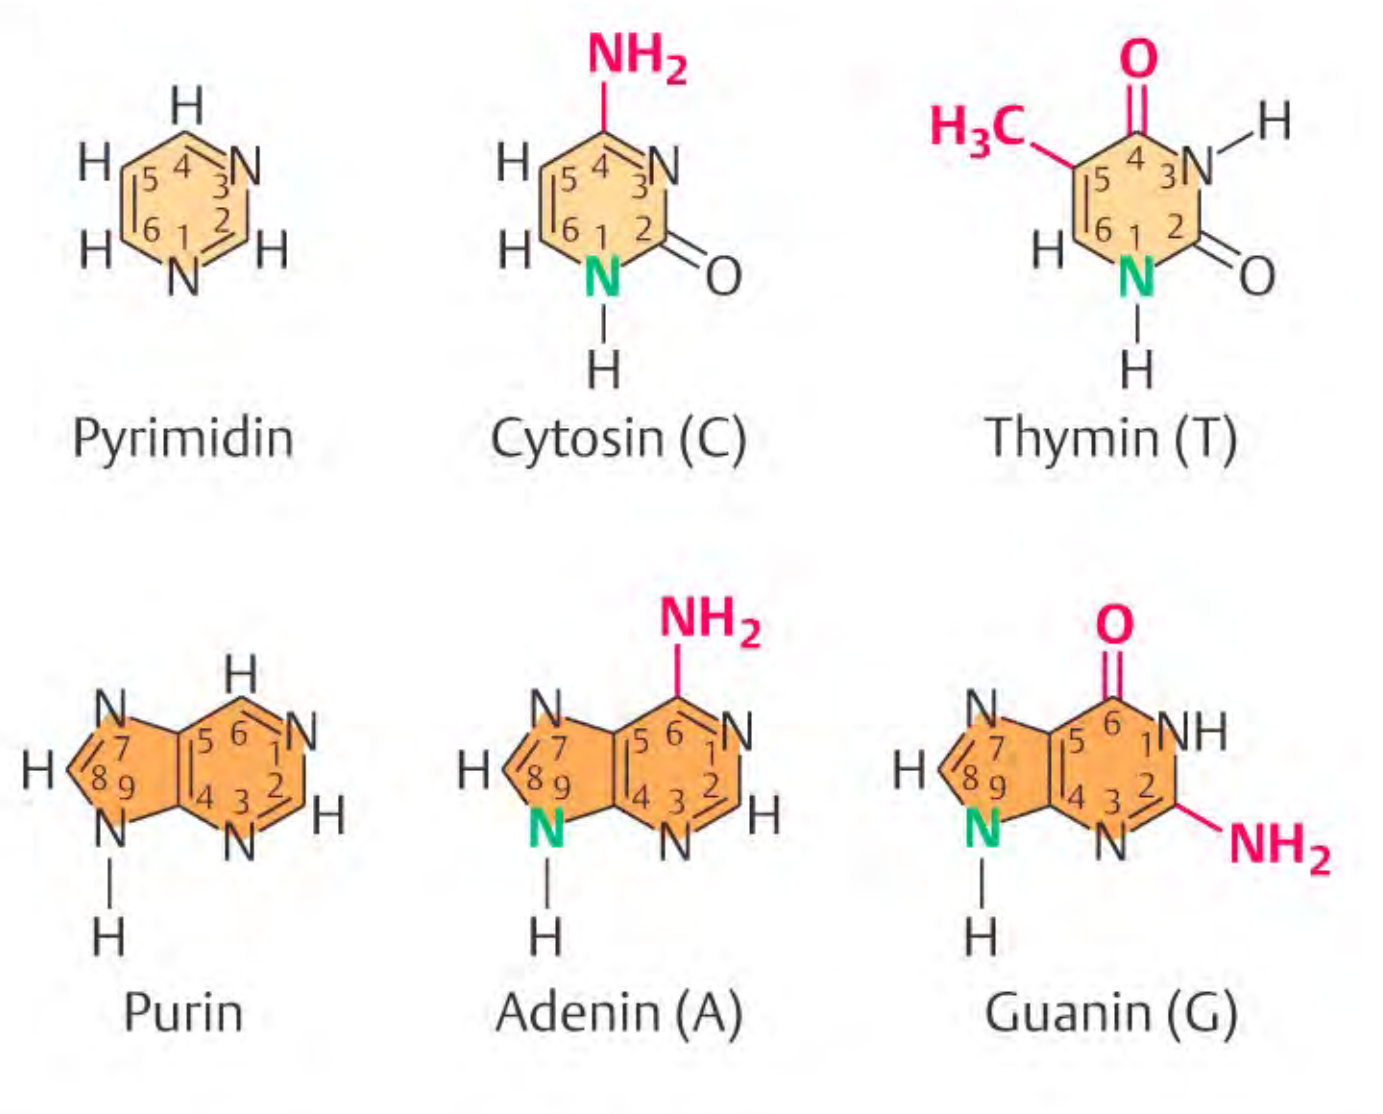
\includegraphics[width=\textwidth]{bilder/basen}
    \caption{Die naturwissenschaftliche Methode als Fließdiagramm.}
\end{figure}

% Folie 18 - 20 nicht drin

\section{Die Mendelschen Regeln}

\defin{merkmalsform}

\regel{mendel1}
Die erste mendelsche Regel wird meistens auf ein oder nur wenige Merkmale bezogen.
Es stimmt aber auch für Inzuchtstämme von z.B.\ Mäusen oder für ``Doppelhaploide'' (DH-Linien) bei Pflanzen.
``gleich'' bezieht sich hier auf den Phänotyp und den Genotyp (für die betrachteten Gene).

\begin{bsp}
    \textbf{Farbige Maiskolben} \\
    % TODO BILD
\end{bsp}

\defin{punnett}


% TODO Dieses F1 und F2 schema (u.a. auf F 26) irgendwie mit einbringen

\regel{mendel2}

\begin{bsp}
    \textbf{Wie finden wir heraus, welcher Genotyp bei ``roter Blüte'' als Phänotyp vorliegt?}
    % TODO F 29
\end{bsp}

\defin{rückkreuzung}

\defin{kopplung}

\defin{zweifaktor_kreuzung}

\begin{bsp}
    \textbf{Mendels Kreuzung mit Pisum sativum}
    % TODO F 32
\end{bsp}

\regel{mendel3}


\subsection{Mendel ``molekular gesehen''}

% TODO F 35 - 41

\section{Vererbung}

\subsection{Rezessive Vererbung}
% TODO F 43

\subsection{Dominante Vererbung}
% TODO F 44 - 45

\subsection{Weitere Vererbungsarten}

\defin{co_dominant}
\defin{multiple_allele}

\begin{bsp}
    \textbf{Blutgruppen}
    % TODO F 48 50
\end{bsp}

\defin{pleiotropie}

\defin{polygene_vererbung}

\defin{umwelteinfluss}

\section{Epistasie}
\defin{epistasie}

% TODO F 52